\chapter{Entorn de desenvolupament PyCharm}

PyCharm és un entorn de desenvolupament integrat (IDE) per Python multiplataforma (Linux, Mac OS i Windows). Per descarregar PyCharm anem a la pàgina de descàrregues de \href{http://www.jetbrains.com/pycharm/download}{JetBrains} i seleccionem la nostra plataforma. PyCharm té moltes característiques interessants pel desenvolupament ràpid d'aplicacions en Python com
autocompletat, autoidentació, control de versions integrat, depurador, refactoring o suport pel testing.


\section{Creant un projecte}

Al crear un projecte hem d'especificar el nom del projecte, que serà el nom de la carpeta; la ruta del projecte dintre del sistema de fitxers i quin intèrpret usarem. Anem a \emph{File - New project} i emplenem el diàleg.

\begin{figure}[!h]
    \begin{centering}
    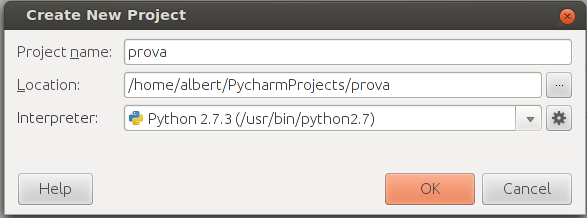
\includegraphics[width=0.7\textwidth]{img/projecte.png}
    \caption{Terminal de Python}
    \label{fig:projecte}
    \end{centering}
\end{figure}


Fent click al projecte creat li diem \emph{File - New} o cliquem a sobre del projecte amb el botó dret i li diem \emph{New}. En ambdós casos seleccionem \emph{Python file} tal i com es mostra a la Fig. ~\ref{fig:nou-fitxer}.


\begin{figure}[!h]
    \begin{centering}
    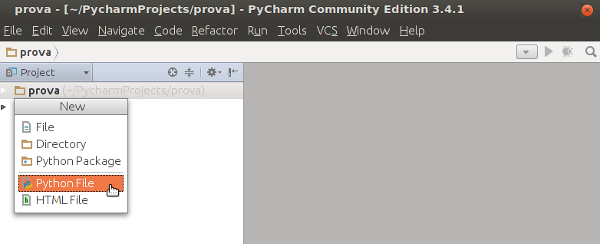
\includegraphics[width=0.9\textwidth]{img/now_fitxer.png}
    \caption{Nou fixer Python}
    \label{fig:nou-fitxer}
    \end{centering}
\end{figure}

Emplenem el nom del fitxer (Fig. ~\ref{fig:main}, que serà l'arxiu \emph{.py} que crearem dins del sistema i que editarem.


\begin{figure}[!h]
    \begin{centering}
    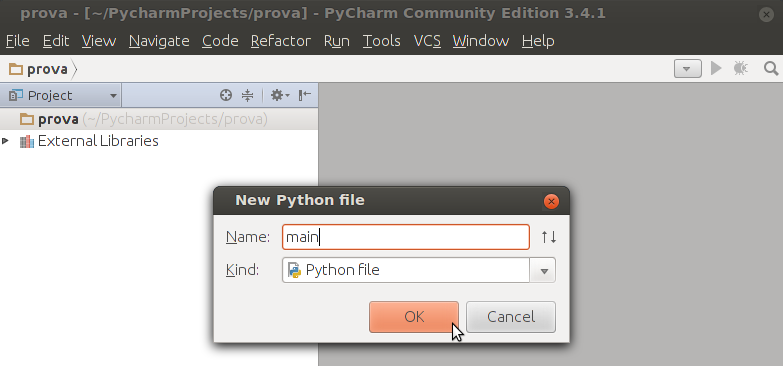
\includegraphics[width=0.9\textwidth]{img/main.png}
    \caption{Emplenar nom del fitxer}
    \label{fig:main}
    \end{centering}
\end{figure}





\section{Executant}


Tenim diverses possibilitats per executar el nostre codi Python. PyCharm inclour l'opció d'execució des de la IDE, també integra la terminal, des de la qual podem cridar al codi, o bé, fins i tot, podem seleccionar el codi amb el cursor, clickar amb el botó dret i seleccionar l'opció \emph{Execute Selection in Console}. En l'exemple mostrat a continuació s'ha usat el següent codi



\begin{blockcode}
import numpy as np

def mitjana(tamany):
    v = np.random.rand(tamany)
    res = np.mean(v)
    return res

print(mitjana(1000))
\end{blockcode}

Després d'haver creat el projecte podem programar directament a l'espai d'edició. Pycharm sagnarà el nostre codi automàticament de tal manera que no haguérem d'estar constantment tabulant cada línia. Per a poder executar el codi anem a Run - Run. Aquesta acció executarà el nostre codi



\begin{figure}[!h]
    \begin{centering}
    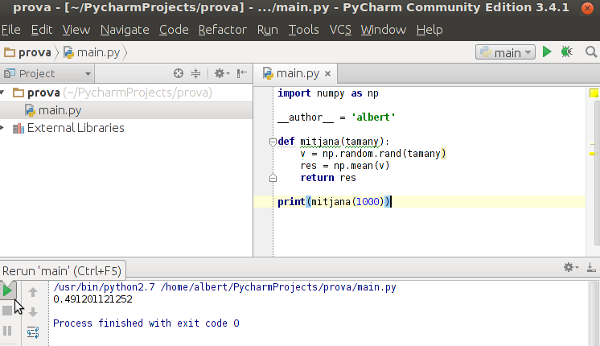
\includegraphics[width=0.9\textwidth]{img/run.png}
    \caption{Execució d'un programa amb PyCharm}
    \label{fig:run}
    \end{centering}
\end{figure}




PyCharm integra la terminal iPython per a que podem treballar amb ella mentre estem desenvolupant el nostre codi. Per defecte la ruta del intèrpret serà la nostra carpeta de treball, així que podem importar amb la comanda {\tt import} el nostre fitxer i cridar les seves funcions tal i com es mostra a la Fig. ~\ref{fig:icharm}.


\begin{figure}[!h]
    \begin{centering}
    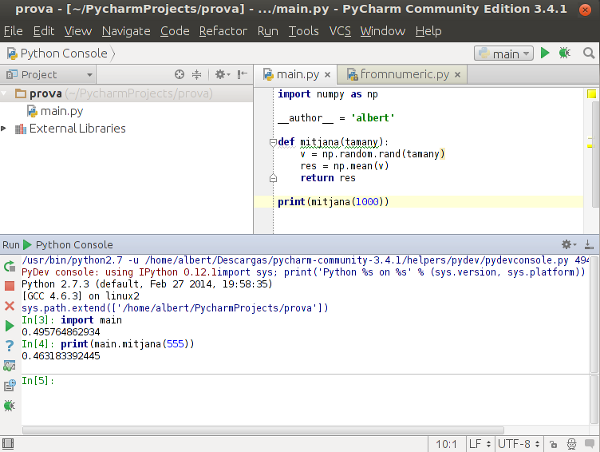
\includegraphics[width=0.9\textwidth]{img/icharm.png}
    \caption{iPython integrat en PyCharm}
    \label{fig:icharm}
    \end{centering}
\end{figure}





Per a depurar el nostre codi anirem a Run - Debug. Abans d'executar-lo el que hem de fer és introduir un \emph{breakpoint}. Per inserir-lo hem de clickar a l'àrea on es troba el punt vermell a la Fi. ~\ref{fig:debug} i seleccionant la línia de codi on volem que s'aturi el codi. Per a avançar en el codi premerem els botons que hi han a l'àrea on es troba el cursor. Al col·locar-nos a sobre veurem la llegenda que ens explica la funcionalitat. Trobarem diverses:

\begin{itemize}
\item \emph{Run to cursor}: executa el codi fins la posició del cursor.
\item \emph{Step into}: entra dintre de la definició de la funció.
\item \emph{Step over}: executar fins la següent línia del mètode on estem
\item Quan volem parar l'execució haurem de prémer el botó quadrat vermell de l'esquerra o fer Ctrl + F2.
\end{itemize}




Trobarem dues pestanyes dintre del marc de depuració de Pycharm. Una s'anomena \emph{Debugger} i l'altre s'anomena \emph{Console}. Quan vulguem veure els resultats que el nostre programa estigui mostren per pantalla haurem d'anar a \emph{Cosole}.


\begin{figure}[!h]
    \begin{centering}
    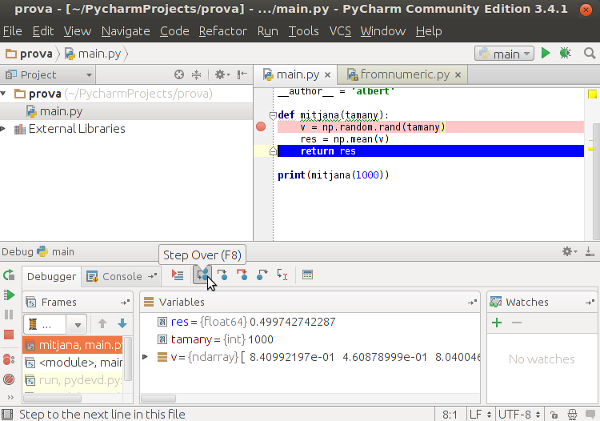
\includegraphics[width=0.9\textwidth]{img/debug.png}
    \caption{Depurant codi Python}
    \label{fig:debug}
    \end{centering}
\end{figure}




\section{Draceres útils}

Les dreceres de teclat ens permeten realitzar accions que incrementen el temps de la nostra productivitat quan treballem. D'altra banda, de vegades hi han més de les que es poden recordar. A continuació es mostra un petit llistat que pot ser d'utilitat.

\begin{itemize}
\item Per a mostrar totes les opcions per autocompletar utilitzem les tecles {\tt Ctrl + espai}

\item Per veure la documentació d'un símbol pressionar {\tt Ctrl + Q}.

\item Per navegar a la declaració d'un símbol premem la tecla {\tt Ctrl} i cliquem a sobre del símbol amb el ratolí.

\item Quan hi ha la llista d'opcions per l'autocompletat premem {\tt Tab} o {\tt Enter} per a seleccionar-la.

\item Quan estem definint una funció i ens trobem amb el cursor entre els parèntesis, al pressionar {\tt Ctrl + P} veurem la paràmetres vàlids.

\item Podem canviar entre pestanyes d'edició amb {\tt Ctrl + Tab}.

\end{itemize}


\subsubsection*{Exercici \Roman{exercici}} \stepcounter{exercici}

Agafant exercicis programats en sessions anteriors:

\begin{itemize}
\item Crear un nou projecte
\item Executar des de la IDE
\item Executar el codi des de iPython
\item Introduir comentaris al nostre codi i després anar a la definició de les nostres pròpies funcions.
\item Anar a les definicions de les funcions cridades
\item Introduir breakpoints i depurar el codi
\end{itemize}
